%% Developing a solution for multimedia home networking chapter
%% author Liu Peng

To fulfill the need of interoperability between devices in home networking,
Tuxera Inc. started a project called Streambels(now called AllConnect). Which
aims to solve the interoperability issue in multimedia home networking. The
solution is to make a combination of most popular solutions into one and
connect all the resources and displays in home. 

Since the hardware and networking settings are not easily changeable. And
nowadays smart phone has great CPU power and networking capability. Thus, they
are well adopted in people's home and even people's life. It is essential to
develop a mobile application that can be used to control all the multimedia data flow in
home networking. Through one year's development, our team developed an Android
application that can be used to control and connect every multimedia device in
the home. The application is integrated with a simple HTTP streaming server,
AirPlay/ DLNA/ Chromecast/ FireTV device discovery, and
AirPlay/ DLNA/ Chromecast/ FireTV streaming control point.

\subsection{Architecture overview}
The architecture of the solution is basically a combination of the most popular
solutions' solutions into one. The whole architecture contains three parts:
discovery, content management and streaming. 

Discovery component is responsible for device discovery which takes advantage of
both Multicast DNS and Simple Service Discovery Protocol. As discussed in
\ref{upnp}, the UPnP service uses Simple Service Discovery Protocol for device
discovery, the application firstly send a M-Search request over UDP to the
IPv4 multicast address 239.255.255.250 and UDP port 1900. Then the application
listen to other devices' response. DIAL devices will return a response with
Application URL header, while the UPnP/DLNA devices will return a message with
a XML body, which gives detailed service URL and description URL. SSDP is used
for both DLNA discovery and DIAL discovery. Multicast DNS is developed and
implemented by Apple Inc., and there is an open source implementation on its
website.

Content management component is responsible for organizing and
navigating multimedia contents which can be found in the home network. In our
solution, this includes both phone's local storage and DLNA digital media
servers that connected to home network. The sources can be used in all of the
three protocols that we support.

Streaming component is responsible for streaming multimedia content to selected
multimedia receivers, such as TVs, wireless speakers, set top boxes etc. In our
solution, since DLNA, AirPlay video/ photo and Chromecast all use HTTP streaming
while AirPlay music uses RTSP. Two types of media servers are built inside our
application. A RAOP server handles the AirPlay music streaming, a HTTP server
handles all the streaming else.

In order to serve media for all the receivers, two types of serve method need to
be implemented in a HTTP server. Since the DLNA guideline gave detailed
specification how the media file should be served on a HTTP server, the HTTP server should be
flexible to add DLNA specific headers, and should support byte based seeking
operation to enable "seek" action on the receiver side. For receivers other than
DLNA, a basic file server with byte range support will just do the work. After
comparing multiple server implementations on Android, NanoHTTPd is the perfect
library for our need, it is easy to use, Apache licensed, very tiny and
efficient implementation, since it is minimal implemented, so it is also easy to
be modified and add additional headers to be compatible with DLNA receivers.


A simplified version of our implementation is shown in the figure \ref{chart3}
below:
\begin{figure}[htb]
\centering 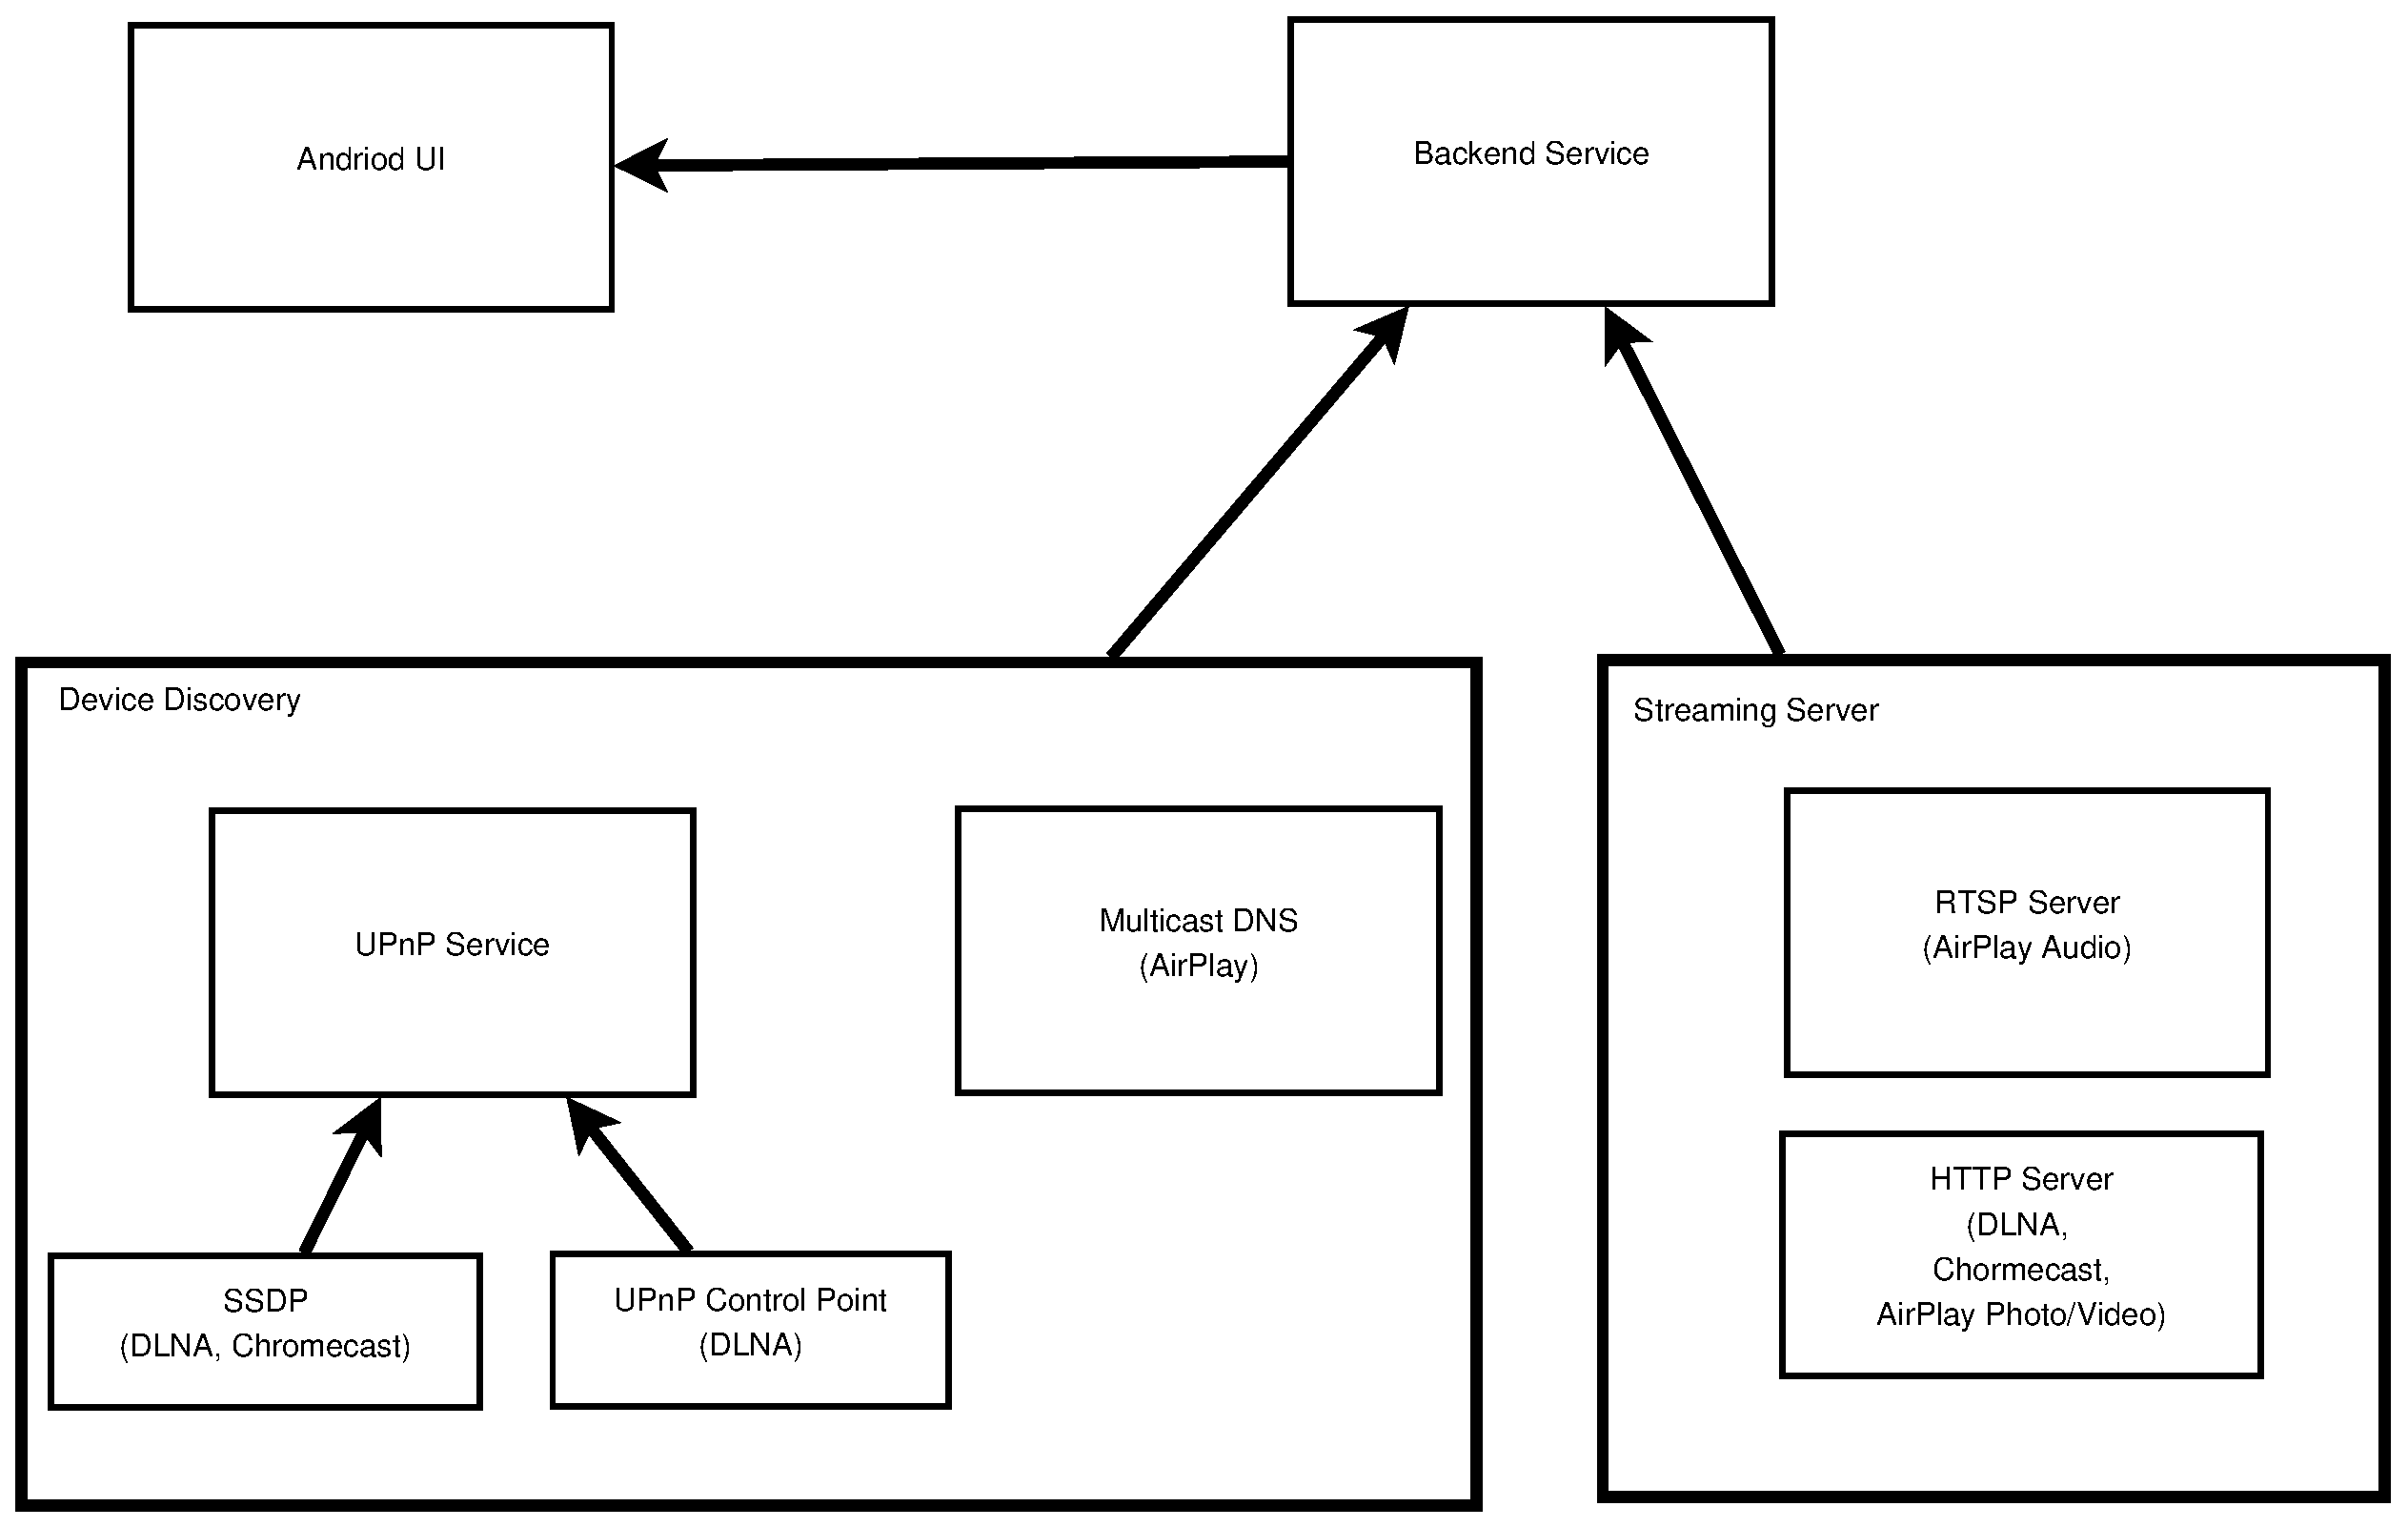
\includegraphics[height=9cm]{charts/chart3}
\caption{Simplified flow chart \label{chart3}}
\end{figure}

In terms of data flow, as described in figure \ref{chart4}, there are three
different types of data flow models: 

If the streamed content is stored in mobile phone, a streaming server in the
application is used to stream the content from phone to selected receiver.

Otherwise, if the content locates on the Internet, and the receiver is a DLNA
Media Renderer, a proxy is needed to firstly download the resource stream, add
the required headers by DLNA protocols and then stream the content to selected
DLNA Media Renderer.

Finally, if the streamed content locates in a DLNA Digital Media Server, the
source can be directly used by all receivers, in this case, the content
streaming happened directly from media server to receivers, application is only
used as a control point and do not participate in the media transmission.

\begin{figure}[htb]
\centering 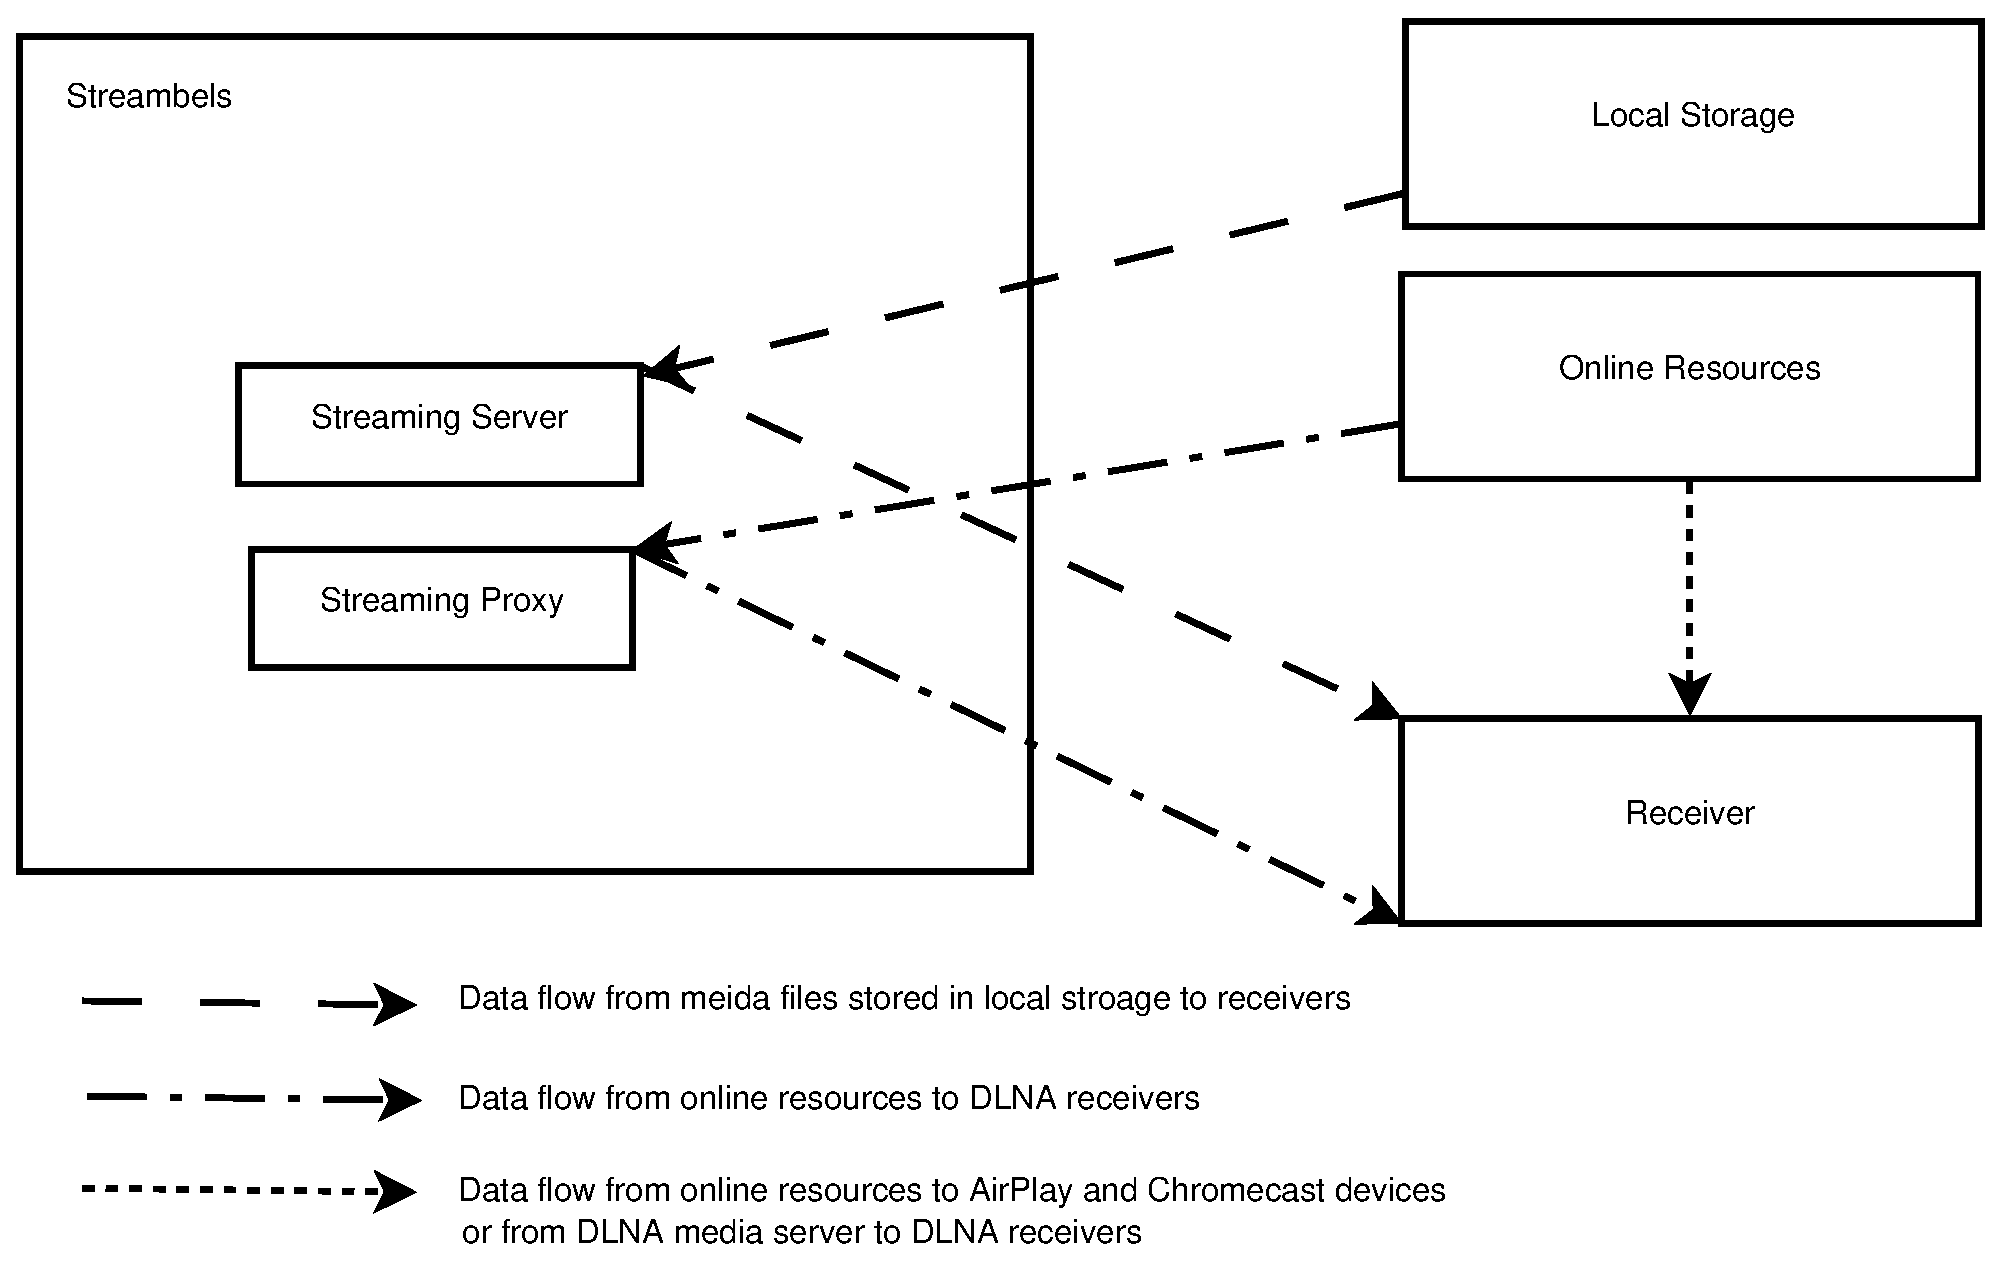
\includegraphics[height=9cm]{charts/data_flow}
\caption{Simplified data flow \label{chart4}}
\end{figure}

In terms of UI and UX, our designer Hien did a great job of defining a simple
and intuitive user interface \ref{chart5}, which benefits a lot for the user
experience.
In every place in the application, selected receiver is visible to user, it is also
visible as a button for switching between different receivers. 9 themes are also
available for users to select, which makes the application more fun to user.
\begin{figure}[htb]
\centering 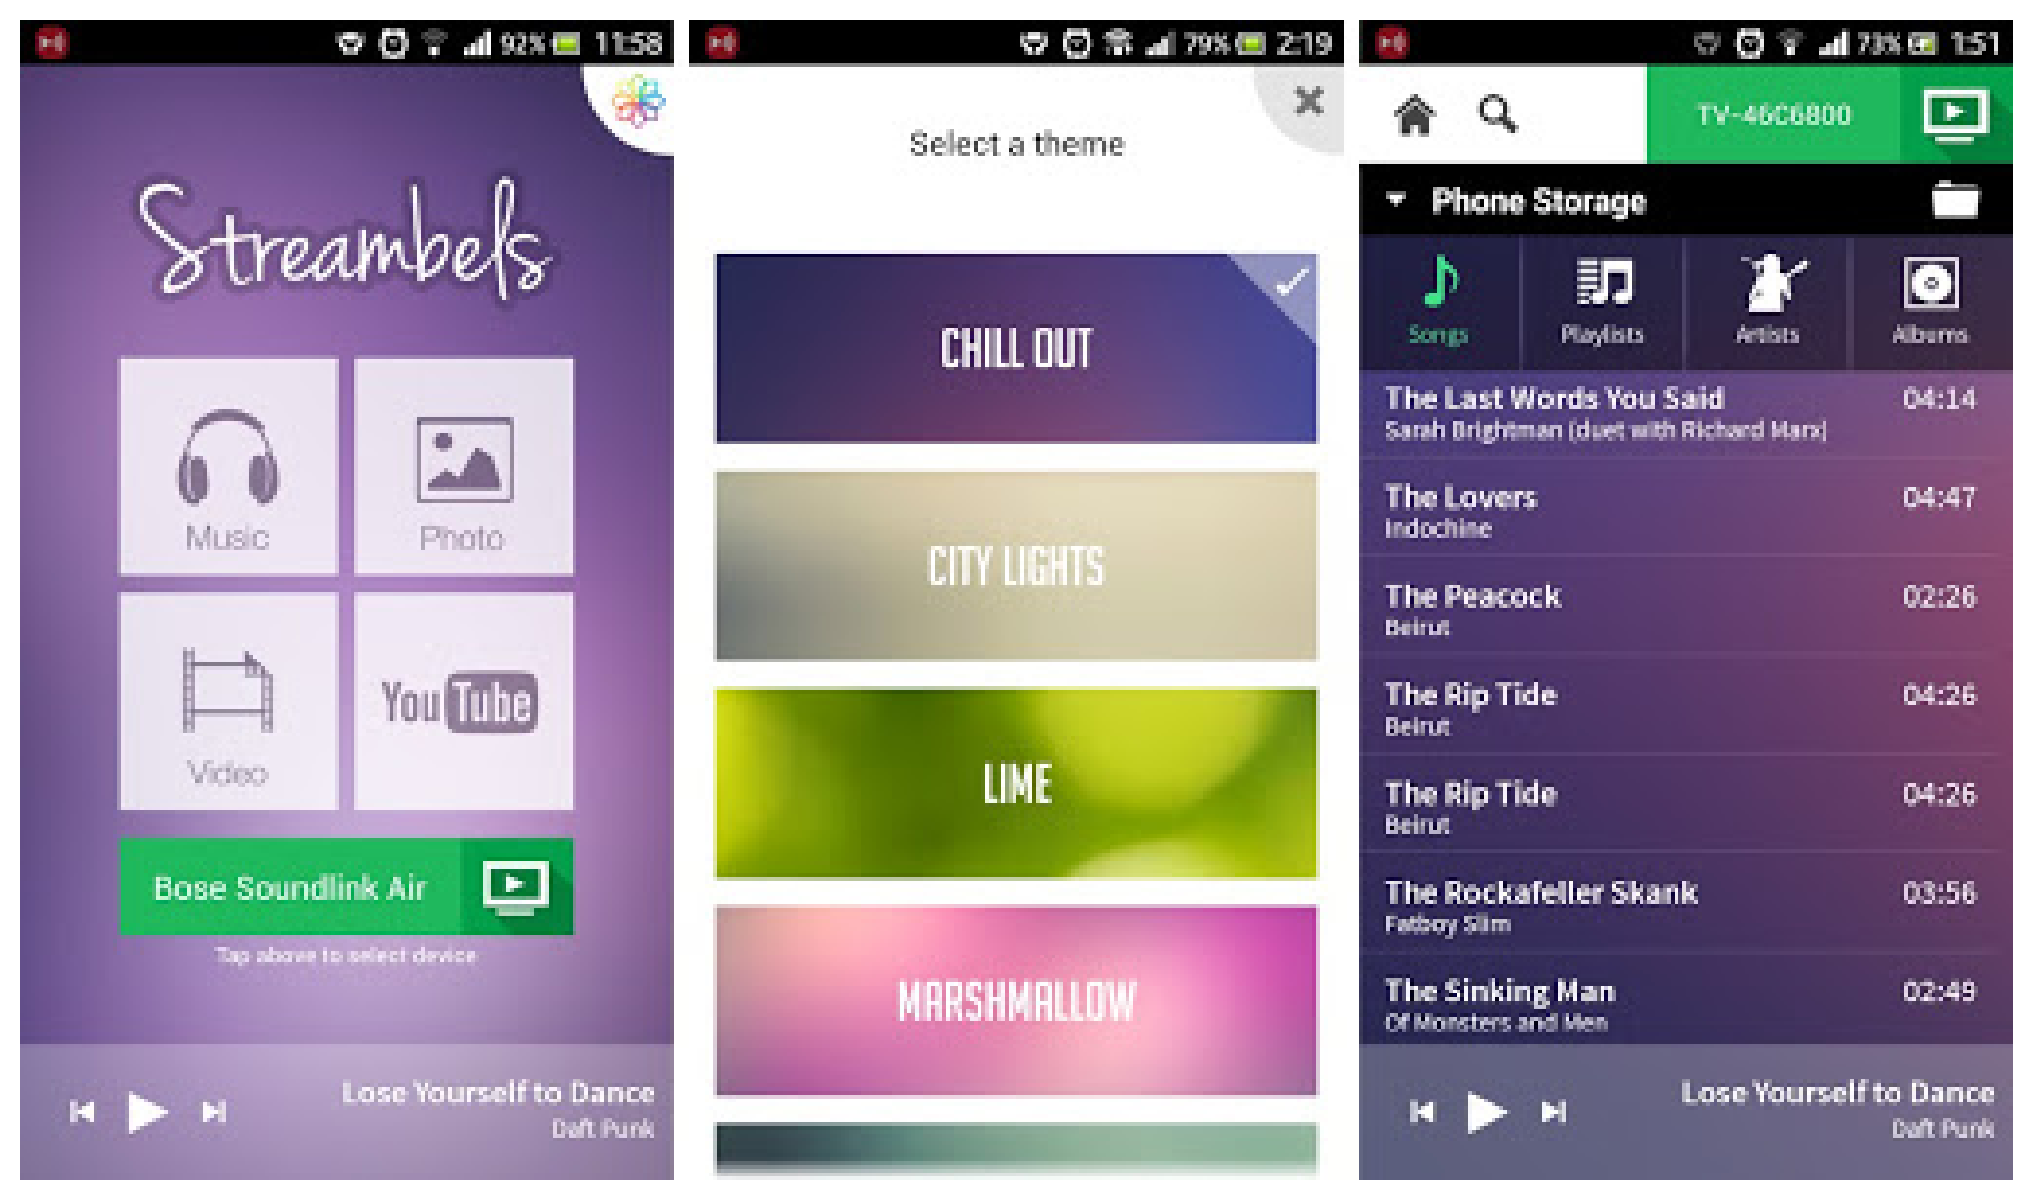
\includegraphics[height=9cm]{charts/streambels_ui}
\caption{Application UX design \label{chart5}}
\end{figure}

\begin{figure}[htb]
\centering 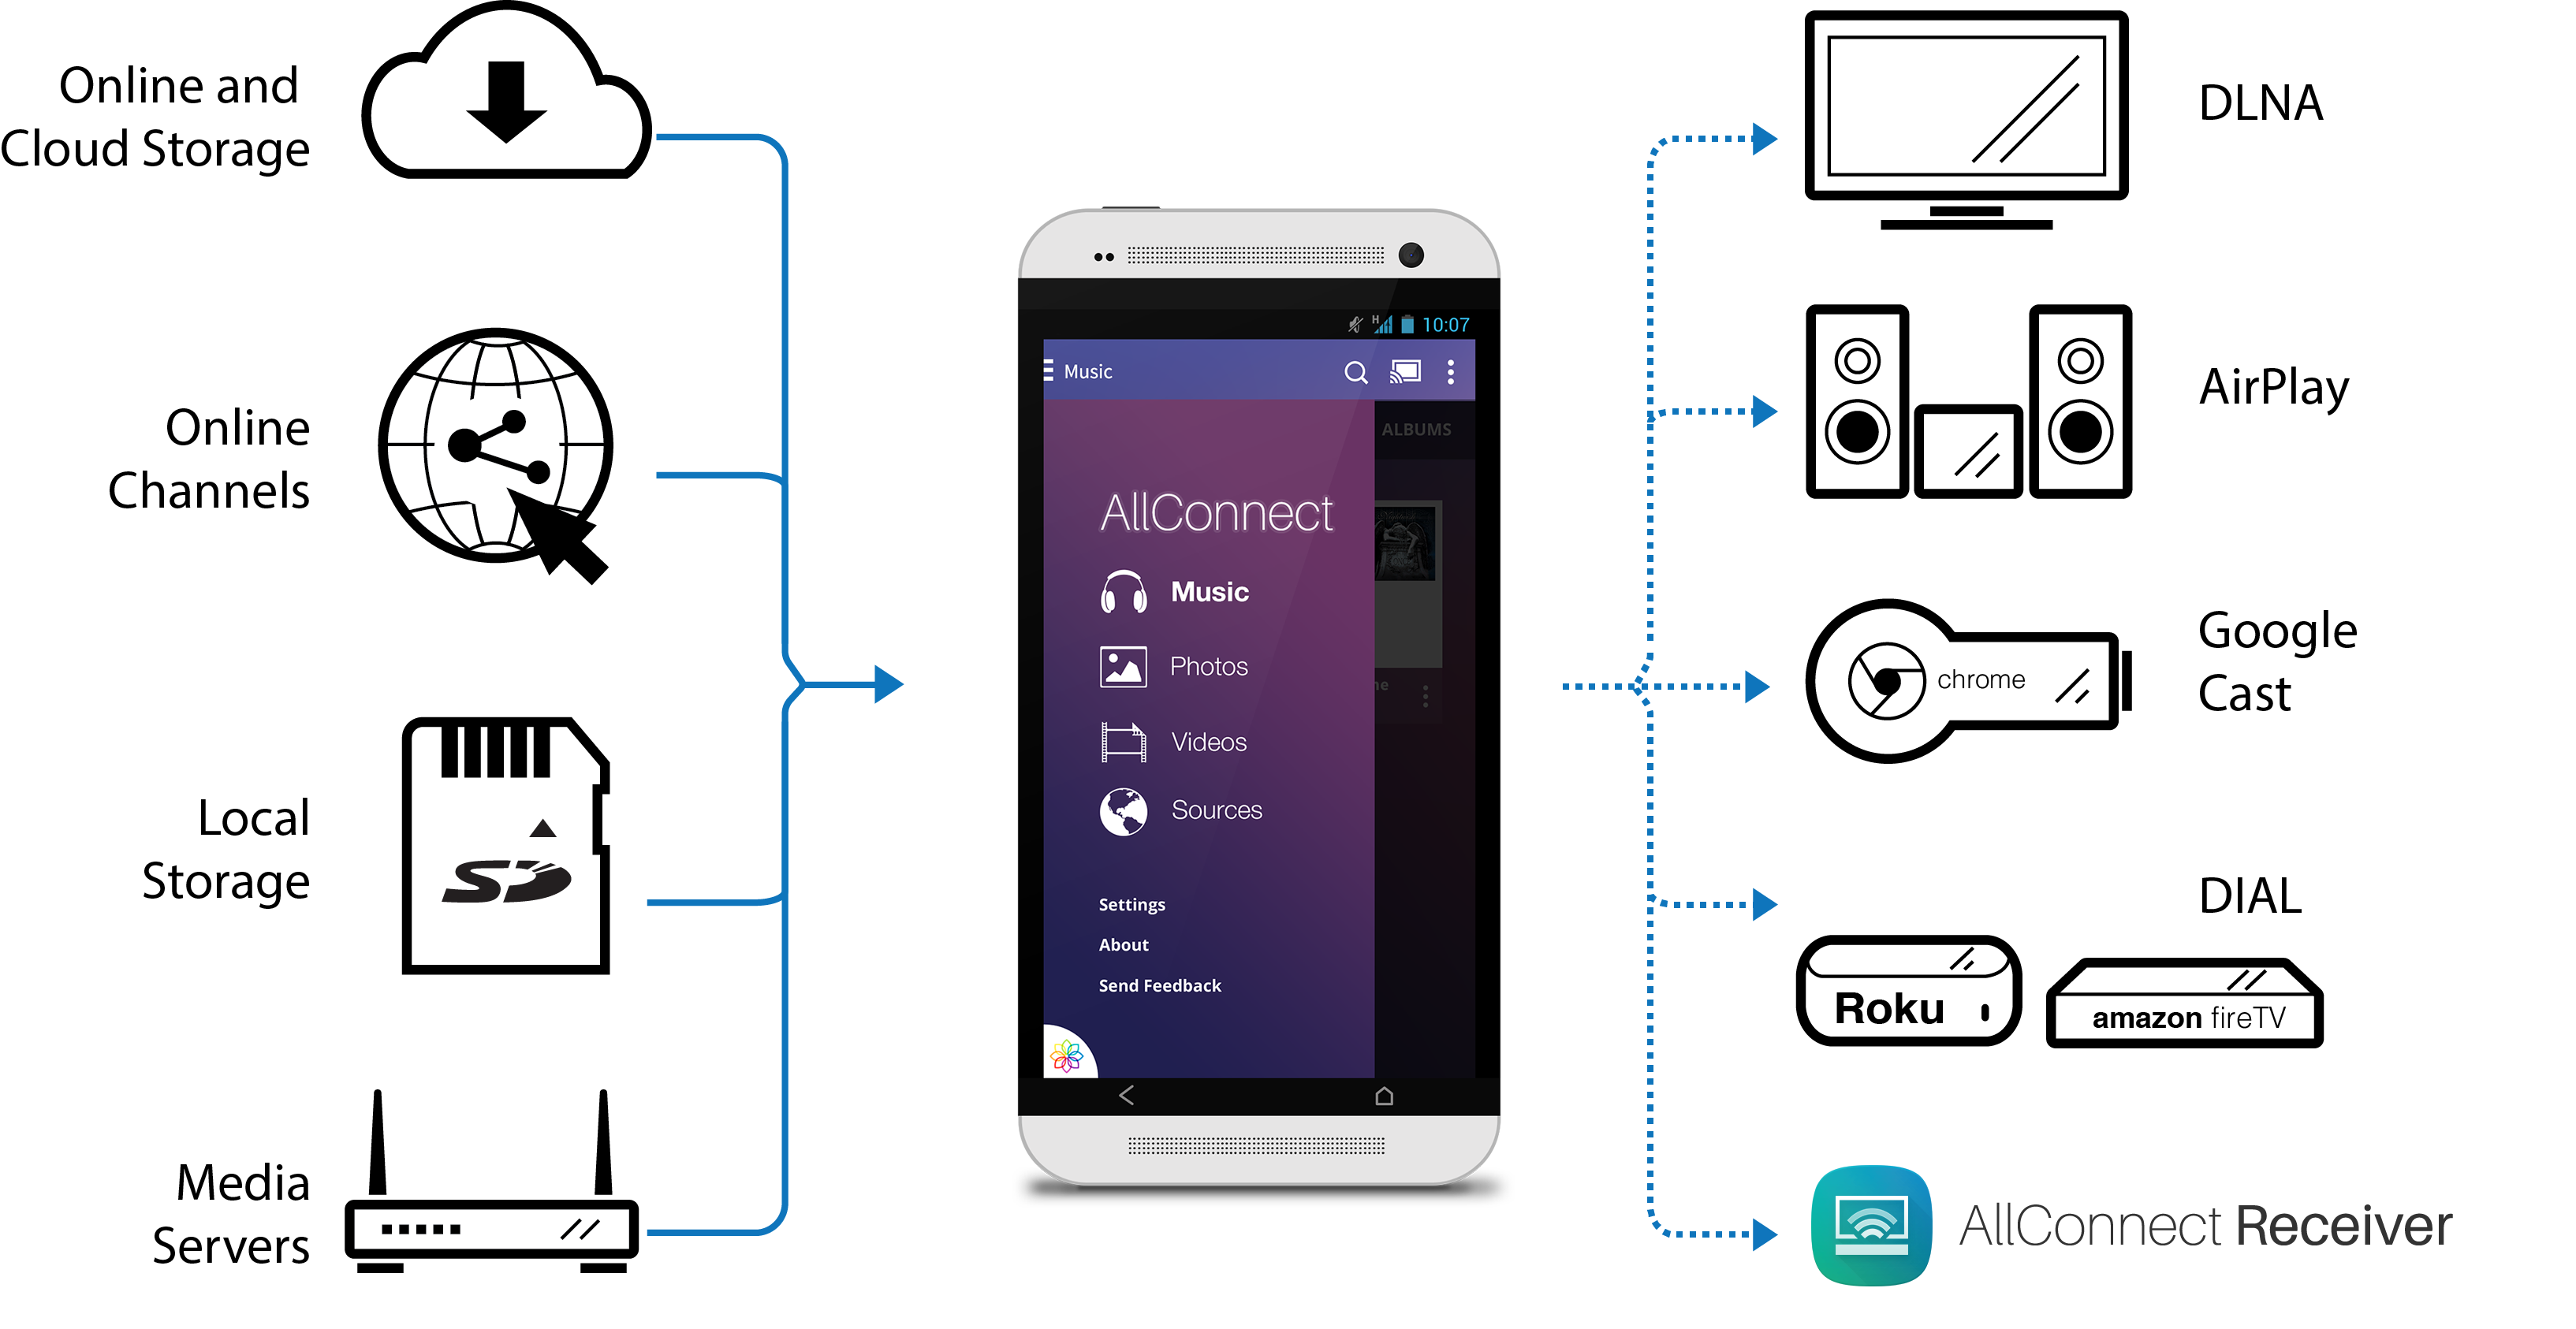
\includegraphics[height=9cm]{charts/allconnect-app}
\caption{Application UX design \label{chart5}}
\end{figure}

\subsection{Features}
As described previously that AirPlay, DLNA and other standards work
differently and have different features, but according to the previous study,
we could combine some common use cases of both protocols.

The Android application we developed can handle most multimedia devices in 
a typical home networking. It has various features that make it a useful and
universal solution for multimedia home networking.

Firstly, the app itself is a multimedia playing, all media stored locally on the
phone storage and all media located in the home DLNA media servers can be
browsed and played on the phone.

Secondly, the app is fully compatible with AirPlay, DLNA, Chromecast and FireTV
receiver devices. 

Thirdly and most importantly, the application make the DLNA media server works
together with all kind of receivers regardless of protocol used. The app served
as a bridge of different multimedia receivers and media sources.

Last, YouTube and other on-line channels like Vimeo and Facebook are supported
as media source, and can be streamed regardless of protocol to all supported
receivers that are connected to home network.


\begin{itemize}
\item[--]Firstly the app is a multimedia player, it can play music, photos and videos 
on SD card locally on Android phone
\item[--]It can stream local content to Apple TV, Airport express and AirPlay-enabled 
speakers.
\item[--]It can stream local content to DLNA media renderers, which has a huge device 
base.
\item[--]It can stream local content to Chromecast devices.
\item[--]It can browse content from the DLNA media servers, a typical source is a 
Network Attached Storage (NAS). And play the media locally on the Android device.
\item[--]It can browse content from the DLNA media servers and stream it to DLNA media 
renderers.
\item[--]It can browse content from DLNA media servers and stream it to AirPlay enabled 
devices using a different protocol.
\item[--]It can proxy online channels' content to DLNA and AirPlay enabled devices. 
(Currently YouTube and Facebook videos are supported, but integration to Spotify is still 
in progress).
\end{itemize}

\subsection{Extensibility}
In normal use cases, the data flow can be shown as figure \ref{chart4},
Streambels has embedded a media streaming server for local files and streaming
proxy for bridging the gap between online resources and home networking. By
using built-in proxy, Streambels is able to share on-line resources from
Internet to devices in home networking environment. New services and new
content providers can be easily added by just call the proxy interface.

The proxy system enables a huge extensibility possibility, which connects the
home networking and Internet or Cloud Services.

Further development abstracted all the protocols and developed an API for all
content holders or cloud services to integrate their service.

\subsection{Test methodology}
Software testing is quite important for a modern IT project. Through testing we
can assure performance and stability, before releasing the app to App store, we
conduct a series of tests.

These tests include unit test, integration test and functional test.
Unit tests is written while coding, when each class is finished, unit tests will
be written for each method, we set up an continuous integration server so that
each time when we commit something to the git repository, a full unit tests will
be run and if there were some failure in the unit tests, developer will be
informed. Integration is done in a way that we ensure each function module
should work together with other modules in the system. Last, we listed all the
possible use cases, prepared a huge media base which contains all kind of media
files, we do manual test before the app is finally released in the market.

\subsection{Evaluation methodology}
Since the project is targeted to Android market, and is directly used by
end users, feedback is really important to us for the continuous development. We
used Email for normal communication, user can edit feedback content directly
inside the application, and later content is sent to us by email.

There is no perfect application, so crash sometimes happen, thanks to Google,
the Google will help to collect the crash reports and show it inside developer
console.

Inside Streambels, we also used Google's Analytics API, which give us
great convenience to collect number of users and sessions every day. Other
information like operation system version, application version, active users
helped us to have insights into who are our users and how can we market for more
people in the world.

It is also interesting to see what kind of technologies are most used in their
daily life, thanks to Google's analytics SDK, we can trigger events when user
selected their receivers, so after months of statistics, we can figure out the
most popular standards and most popular online channels that user uses, and in
turn make better optimizations for users need.


